\chapter{Discussion}
\label{sec:discussion}
Chapter 4, 5 and 6 introduce to create an \gls{rl}

\section{Guaranteeing safety}
\label{sec:system_architecture}
Safety is the most important factor of a \gls{ad} system, but since \gls{rl} is a data driven approach it is very difficult to guarantee safety \cite{tbd} in the same way e.g., a \gls{mpc} can. That is why this section will clarify where the work in this thesis would fit in by first defining a system architecture for \gls{ad}, its modules and a short summary of the ISO 26262 standard. Then, place itself within the system and motivate how safety can be guarantied. 

The architecture of an autonomous driving system can be divided into perception, planning and control~\cite{Schwarting2018,Kortenkamp2008}.
The perception module is responsible for sensing and mapping the environment with the use of sensors such as LIDARs, cameras, radars etc. The raw data from the sensors are then processed though various sensor fusion techniques to generate a representation of the environment, e.g., position, velocity of other traffic participants while also describing the road such as width and distance to the next intersection. This information is then used by the planner to create a driving strategy of how to transverse through the world. However, the information from the sensors are often noisy, with false positives and false negatives making it difficult for the planner.

Tactical planning can be divided into three categories, the proactive, active and reactive. A proactive module would be something like a precautionary safety module that interprets the information about the environment and create constraints that is sent to the active planner, like  driveable area, allowed speeds and actions. These constraints are generated from a set of safety goals and rules, making this the first layer of protection that can ensure safety. 
The role of the active planner is to take this sets of allowed actions and prescribe the behavior of the vehicle through decisions such as drive, yield or stop. The goal of these high level decisions is to optimize metrics such as comfort, fuel consumption and time to goal. These decisions are then sent to a motion planner that generates a safe dynamically feasible path for the vehicle for a shorter planning horizon of around $0.1$s. 
At the same time, a reactive, collision avoidance, module make sure that the chosen decision and path does lead to any collisions. Unlike the decision maker, the collision avoidance module main goal is to identify imminent danger and therefore has access to more aggressive actions like emergency breaking to ensure safety. 
 
In the industry today the main standard for functional safety in motorized vehicles is the ISO 26262 standard, titled "Road vehicles – Functional safety"~\cite{ISO26262}. It uses a \gls{asil} to classify the inherent safety risk in an automotive system and the functions or modules of such a system. The \gls{asil} classification is used to express the level of risk reduction required to prevent a specific hazard, from \gls{asil} D to \gls{asil} A. \gls{asil} D represents the highest hazard level and \gls{asil} A the lowest. There is a level with no safety relevance and only standard Quality Management processes are required, this level is referred to as QM.

\begin{figure}[h]
	\centering
	 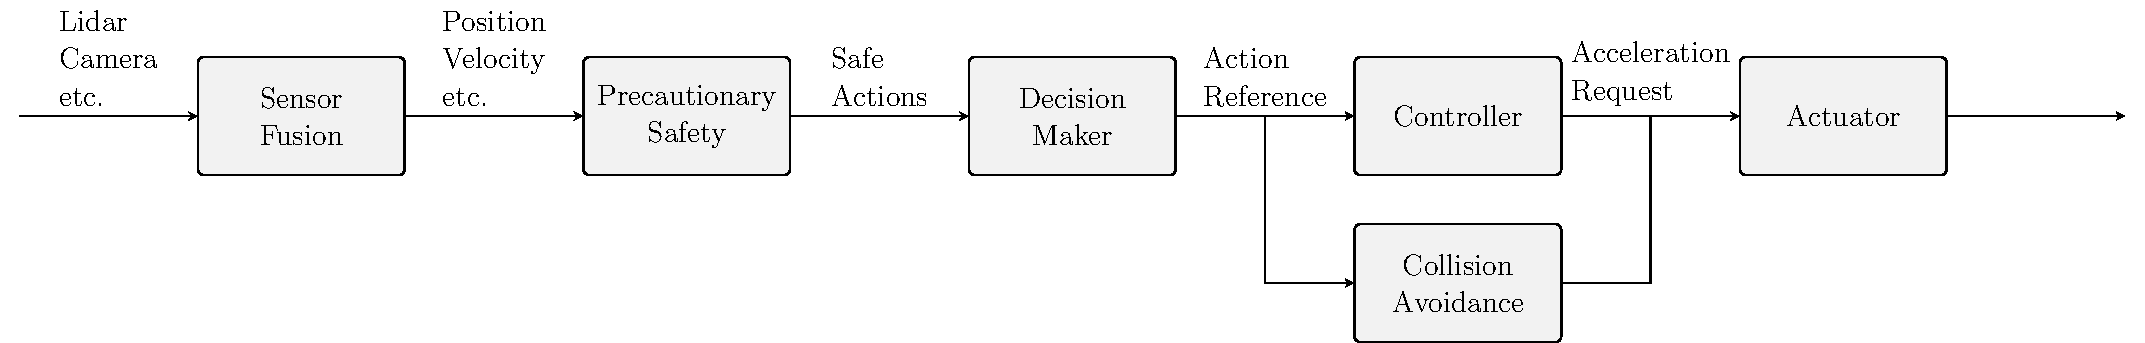
\includegraphics[width=\linewidth]{YourThesis/chapters/figures/pomdp/figures-system_architecture.pdf}
%	\begin{tikzpicture}[
%		node distance=8mm and 30mm,
%		node font= \Large,
%		box/.style = {draw, thick, rectangle, rounded corners=0.1cm, fill=gray!10, minimum width=3.5cm, minimum height=2cm, align=center},
%		sx+/.style = {xshift = 2mm},
%		sx+/.style = {xshift = 2mm}
%		]
%
%		% \node[draw,thick,rectangle,rounded corners =0.05cm,fill=gray!10,minimum width=2cm,minimum height = 2cm] (SF) at (2,0) {Sensor Fusion};
%		
%		% \draw[arrow,thick] (0,0) --(SF) node [midway,above] {Sensors: Lidar, Radar, Camera, Sonar};
%
%		% \node[draw,thick,rectangle,rounded corners =0.05cm,fill=gray!10,minimum width=2cm,minimum height = 2cm, shift={(2,0,0)}] (SF) at (2,0) {Sensor \\ Fusion};
%		
%		\node (start) at (0,0) {};
%		\node (SF) [box, right=of start.east] {Sensor \\ Fusion};
%		\node (PS) [box, right=of SF.east] {Precautionary \\ Safety};
%		\node (DM) [box, right=of PS.east] {Decision \\ Maker};
%		\node (Con) [box, right=of DM.east] {Controller};
%		\node (CA) [box, below=of Con] {Collision \\ Avoidance};
%		\node (Act) [box, right=of Con.east] {Actuator};
%		\node (end) [right=of Act] {};
%
%		\draw[arrow,thick,align=left] (start) --+(SF) node [midway,above] {Lidar\\Camera\\etc.};
%		\draw[arrow,thick,align=left] (SF) --+(PS) node [midway,above] {Position\\Velocity\\etc.};
%		\draw[arrow,thick,align=left] (PS) --+(DM) node [midway,above] {Safe\\Actions};
%		\draw[arrow,thick,align=left] (DM) --+(Con) node [midway,above] {Action\\Reference};
%		\draw[arrow,thick,align=left] (DM) -| ($(DM.east) + (1.5,0mm)$) |- (CA) node [midway,above] {};
%		\draw[arrow,thick,align=left] (CA) -| ($(CA.east) + (1.5,0mm)$) |- (Act) node [midway,above] {};
%		\draw[arrow,thick,align=left] (Con) --+(Act) node [midway,above] {Acceleration\\Request};
%		\draw[arrow,thick,align=left] (Act) --+(end) node [midway,above] {};
%	% --> Sensor Fusion --> Precautionary Safety --> |Decision Maker --> Controller |--> Actuator -->
%	% 																->Collision Avoidance |
%
%	\end{tikzpicture} 
	\caption{Representation of the system architecture.}
	\label{fig:system_architecture}
\end{figure}

Although safety is the most important requirement for enabling autonomous driving, the work in this paper does not make any safety guarantees. Instead, it is proposed that the decision-making algorithms presented in this paper be used in the system architecture shown in Figure~\ref{fig:system_architecture}. This approach allows higher \gls{asil} to be applied to the precautionary safety and collision avoidance modules, while the decision-making algorithms focus primarily on comfort. As a result, the \gls{asil} classification for the decision-making components could be at lower levels, potentially even classified as QM in the best case.

% \tommy{To explore different ways to make the driving policy safe and increase the capability of handling uncertainty in the environment. But even so the state of machine learning and neural networks today is still very limited when its comes to guaranteeing safety. Therefore, it is important to have a system architecture that can separate safety guarantees to another module so that the main benefits of using machine learning can be fully utilized.}

% \tommy{To be able to use \gls{ml} and \gls{rl} safety is this stage of development it is important to separate the responsibility of safety to a more capable system like formal methods, reachability or MPC that can mathematically guarantee safety.}
 
% \tommy{depending on size of chapter consider moving it to its own chapter.}
 
% The ASIL assessed for a given hazard is then assigned to the safety goal set to address that hazard and is then inherited by the safety requirements derived from that goal.
% These Severity, Exposure, and Control definitions are informative, not prescriptive, and effectively leave some room for subjective variation or discretion between various automakers and component suppliers.



% This paper aims to sparate the task of ensuring safety to a precautionary safety or collision avoidance module. 

% \todo{include a description of ISO26262, motivate a redundant system for Asil D, making it important to separate the scope of the tactical decision making agent to be comfortable and efficient. Efficiency can be measured in different ways, but in this paper we refer to change in acceleration, number of times the agent reaches an undesired terminal state and the time it takes to reach the goal.}


% \section{Simulation and real world}
% Bridging the gap between simulation and real world. Ever evolving driving styles. Building trust. 

% \section{scalability}
% One big model versus small models. Sovling the general problem of driving vs, special cases. 

% \section{Designning the reward function}